\documentclass[10pt,final,leqno]{beamer}

%\usetheme{CambridgeUS}
\usetheme[style=ntnu,language=en]{ntnu2015}
%\usecolortheme{orchid}

\usepackage[utf8]{inputenc}
\usepackage[T1]{fontenc}

% Paths
\newcommand{\figs}{../figs}
\newcommand{\data}{../data}
\newcommand{\code}{../code}

% URL styles
\usepackage{url}
\urlstyle{sf}

% Units
\usepackage[detect-weight=true, binary-units=true]{siunitx}
\DeclareSIUnit\flop{FLOPS}

% Math
\usepackage{amsmath}
\usepackage{amssymb}
\usepackage{bm}
\usepackage{nicefrac}
\newcommand{\dif}[1]{{\;\text{d}#1}}

% Graphics
\usepackage{graphicx}
\usepackage{caption}
%\usepackage{subcaption}
\graphicspath{{../figs/}}

% Tikz
\usepackage{tikz}
\usetikzlibrary{positioning,shapes,arrows,calc,intersections}
\usepackage{pgfplots}
\usepgfplotslibrary{dateplot}
\pgfplotsset{compat=1.14} 

% Colors
\definecolor{darkblue}{HTML}{00688B}
\definecolor{darkgreen}{HTML}{6E8B3D}
\definecolor{cadet}{HTML}{DAE1FF}
\definecolor{salmon}{HTML}{FFB08A}

\usepackage{algorithm}

% Listings
\usepackage{textcomp}
\usepackage{listings}
\lstset{
  keywordstyle=\bfseries\color{orange},
  stringstyle=\color{darkblue!80},
  commentstyle=\color{darkblue!80},
  showstringspaces=false,
  basicstyle=\ttfamily,
  upquote=true,
}
\lstdefinestyle{fortran}{
  language=Fortran,
  morekeywords={for},
  deletekeywords={status},
}
\lstdefinestyle{c}{
  language=C,
  morekeywords={include},
}
\lstdefinestyle{glsl}{
  language=C,
  morekeywords={attribute, vec2, vec3, vec4, varying, uniform, mat2, mat3, mat4},
}
\lstdefinestyle{cuda}{
  language=C,
  morekeywords={__global__, __device__, __host__, __shared__},
}
\lstdefinestyle{shell}{
  language=bash,
  morekeywords={mkdir, ssh, cmake},
}

% Double hlines
\usepackage{hhline}

% Misc
\usepackage{nth}

\subtitle{TMA4280---Introduction to Supercomputing}

\graphicspath {{../figs/}}

\AtBeginSection[]
{
 \begin{frame}<beamer>
 \frametitle{Outline}
 \tableofcontents[currentsection]
 \end{frame}
}

\begin{document}


%\newcommand{\xC}{\mathbb{C}}
\newcommand{\xR}{\mathbb{R}}
\newcommand{\xRd}{{\xR^d}}
\newcommand{\xRN}{{\xR^N}}
\newcommand{\xMNR}{{M_N(\xR)}}
\newcommand{\bb}{{\boldsymbol b}}
\newcommand{\ee}{{\boldsymbol e}}
\newcommand{\ev}{{\boldsymbol \epsilon}}
\newcommand{\rr}{{\boldsymbol r}}
\newcommand{\xx}{{\boldsymbol x}}
\newcommand{\hx}{\hat{\boldsymbol x}}
\newcommand{\yy}{{\boldsymbol y}}
\newcommand{\vv}{{\boldsymbol v}}
\newcommand{\ww}{{\boldsymbol w}}
\newcommand{\zz}{{\boldsymbol z}}
\renewcommand{\mA}{{\mathrm A}}
\newcommand{\mB}{{\mathrm B}}
\newcommand{\mC}{{\mathrm C}}
\newcommand{\mD}{{\mathrm D}}
\newcommand{\mG}{{\mathrm G}}
\newcommand{\mH}{{\mathrm H}}
\renewcommand{\mL}{{\mathrm L}}
\newcommand{\mLs}{{\mathrm L_0}}
\newcommand{\mM}{{\mathrm M}}
\newcommand{\mRs}{{\mathrm R_0}}
\newcommand{\mR}{{\mathrm R}}
\newcommand{\mP}{{\mathrm P}}
\newcommand{\mQ}{{\mathrm Q}}
\newcommand{\mU}{{\mathrm U}}
\newcommand{\mId}{{\mathbf{Id}}}
\newcommand{\mII}{{\mathbf{\mathbb{I}}}}
\newcommand{\Seq}[1]{\bigl(#1\bigr)}
\newcommand{\Cond}[1]{\mathcal{C}(#1)}
\newcommand{\Order}[1]{\mathcal{O}\left(#1\right)}
\newcommand{\norm}[1]{{\lVert #1 \rVert}}
\newcommand{\norminf}[1]{\norm{#1}_{\infty}}

\newcommand{\InnerK}[2]{{{\mathbf\langle}\;#1\:,\: #2 \;{\rangle}}}
\newcommand{\Inner}[2]{{{\scriptstyle\mathbf{(}}\;#1\:,\: #2 \;{\scriptstyle\mathbf{)}}}}


\title{Parallel I/O with MPI}
\institute{NTNU, IMF}
\date{April 13. 2018}
%\author{Based on 2016v slides by Eivind Fonn}
%\author{Aurélien Larcher}

\maketitle

\begin{frame}
  \frametitle{Limits of data processing}

  \begin{itemize}
  \item Development of computational resource allow running more complex simulations.
  \item Volume of data produced grows in consequence and can become a problem for performance.
  \item Reading and writing data to/from a process is named Input/Output (IO).
  \item Data may be read/written for:
  \begin{itemize}
  \item meshes used as computational domain
  \item saving discrete solution (ex: velocity field for Navier--Stokes)
  \item sampling physical quantities for postprocessing
  \end{itemize}
  \end{itemize}

Nowadays data can be produced at a faster rate than it can be processed.
\end{frame}
%-----------------------------------------------------------------------------

\begin{frame}
  \frametitle{Bottleneck for I/O: Sequential}

\begin{figure}
  \begin{center}
    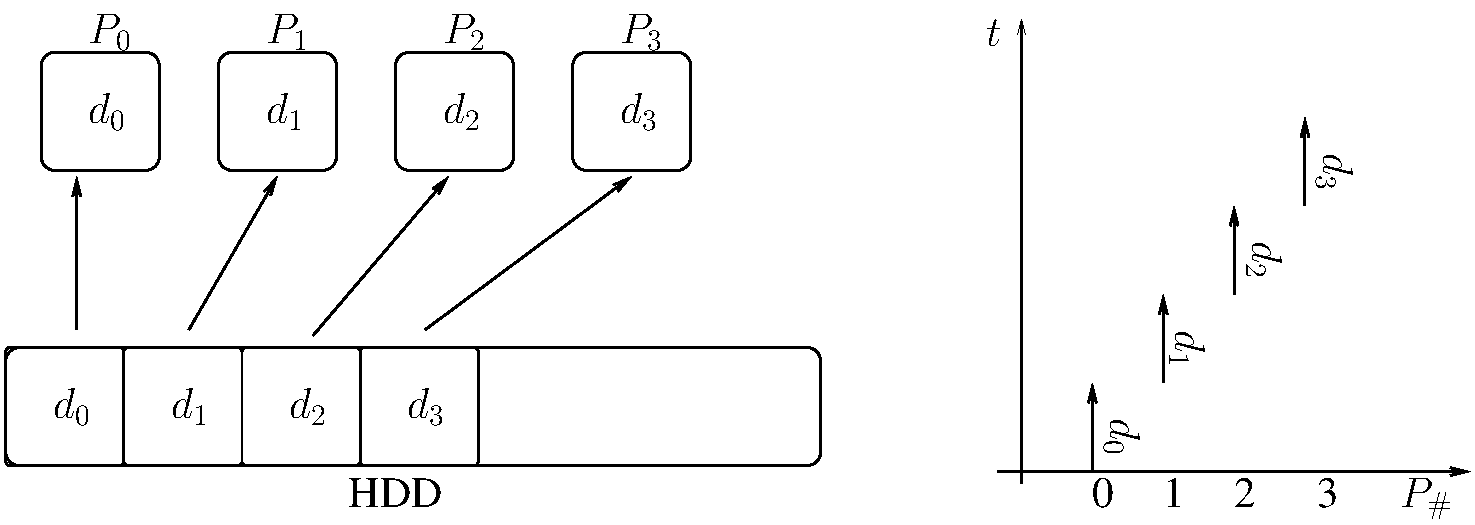
\includegraphics[width=10cm]{\figs/many-onedisk}
  \end{center}
  \caption{
    Illustration of I/O where several processes read from a single file. Since a
    HDD is serial in nature, only one operation can be performed concurrently.
  }
\label{fig:manyone}
\end{figure}
\end{frame}
%-----------------------------------------------------------------------------

\begin{frame}
  \frametitle{Bottleneck for I/O: Parallel}
\begin{figure}
  \begin{center}
    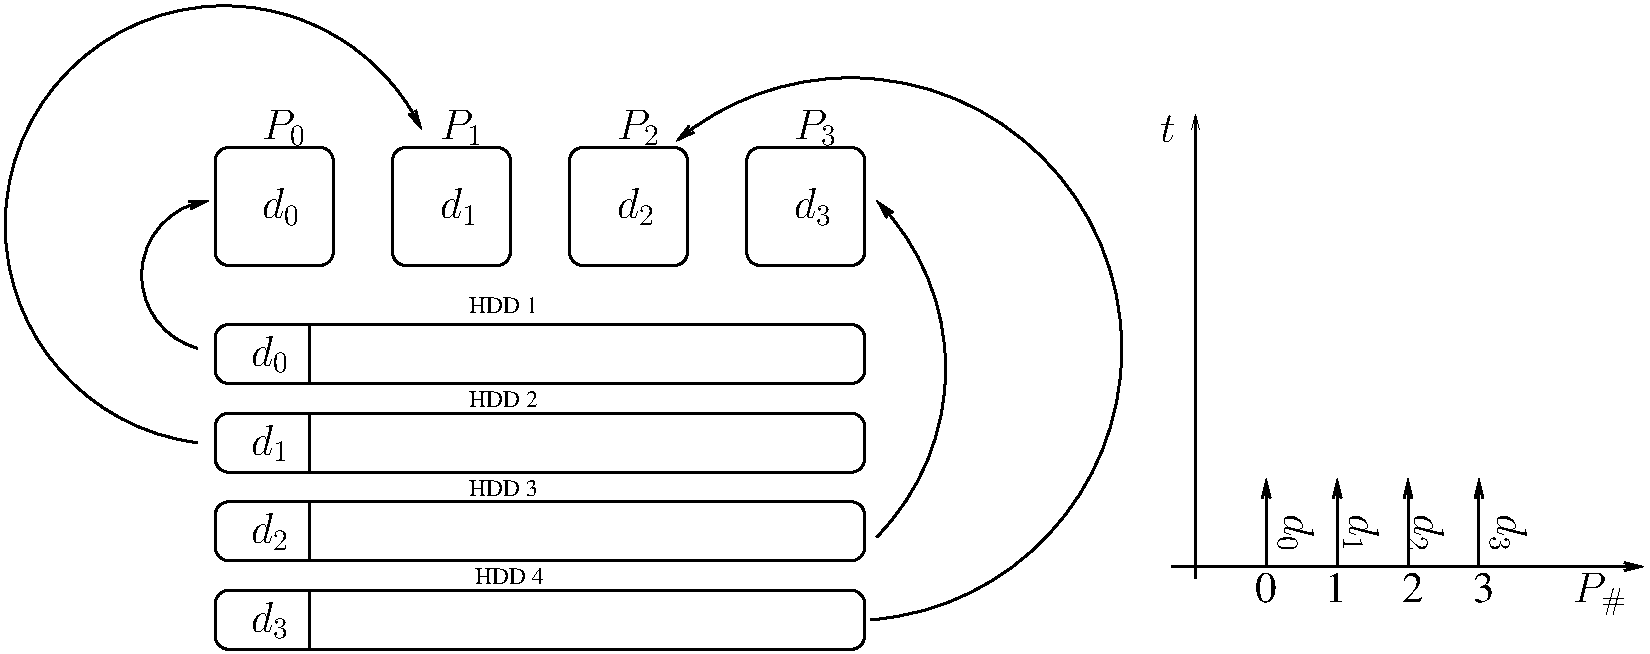
\includegraphics[width=10cm]{\figs/many-manydisk}
  \end{center}
  \caption{
    Illustration of I/O where we harness the aggregated bandwith of several
    devices. Here each process reads its data from a separate physical device,
    thus the I/O can be performed in parallel.
  }
  \label{fig:manymany}
\end{figure}

\end{frame}
%-----------------------------------------------------------------------------

\begin{frame}
  \frametitle{Parallel distributed filesystems}

\begin{itemize}
\item Parallel distributed filesystem are used widely on supercomputers
\item The most popular is Lustre (used for instance by LLNL with ZFS)
\item They offer high-throughput but also fault-tolerance
\item Other popular options are: MooseFS, OrangeFS, GlusterFS.
\end{itemize}

\end{frame}
%-----------------------------------------------------------------------------

\begin{frame}
  \frametitle{Example: Landing Gear Simulation}

\begin{figure}
  \begin{center}
    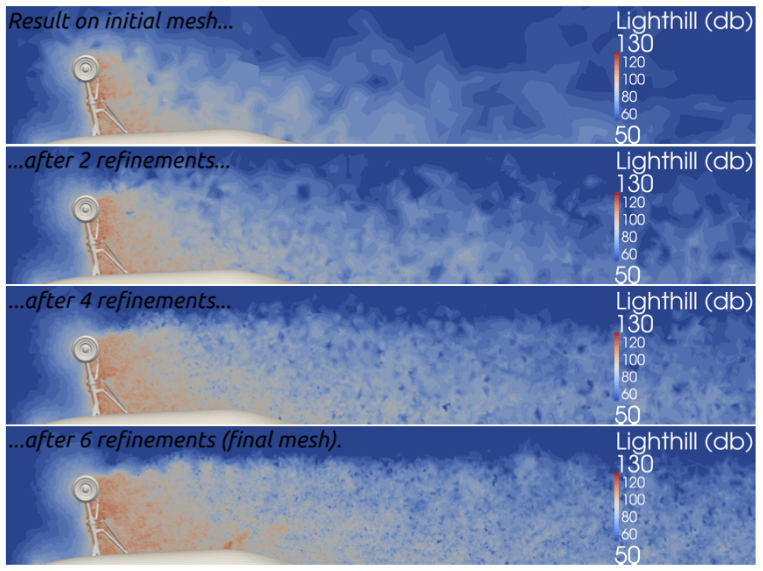
\includegraphics[width=8cm]{\figs/ctl/banc2_stages}
  \end{center}
  \caption{Initial 3.6M elements, Final 23.8M elements (600K core.h).
Vilela De Abreu/N. Jansson/Hoffman, 18th AIAA Aeroacoustics Conference, 2012}
\end{figure}

Lighthill tensor to evaluate noise generation on the landing gear.
\end{frame}
%-----------------------------------------------------------------------------

\begin{frame}
  \frametitle{Example: Landing Gear Simulation}

\begin{figure}
  \begin{center}
    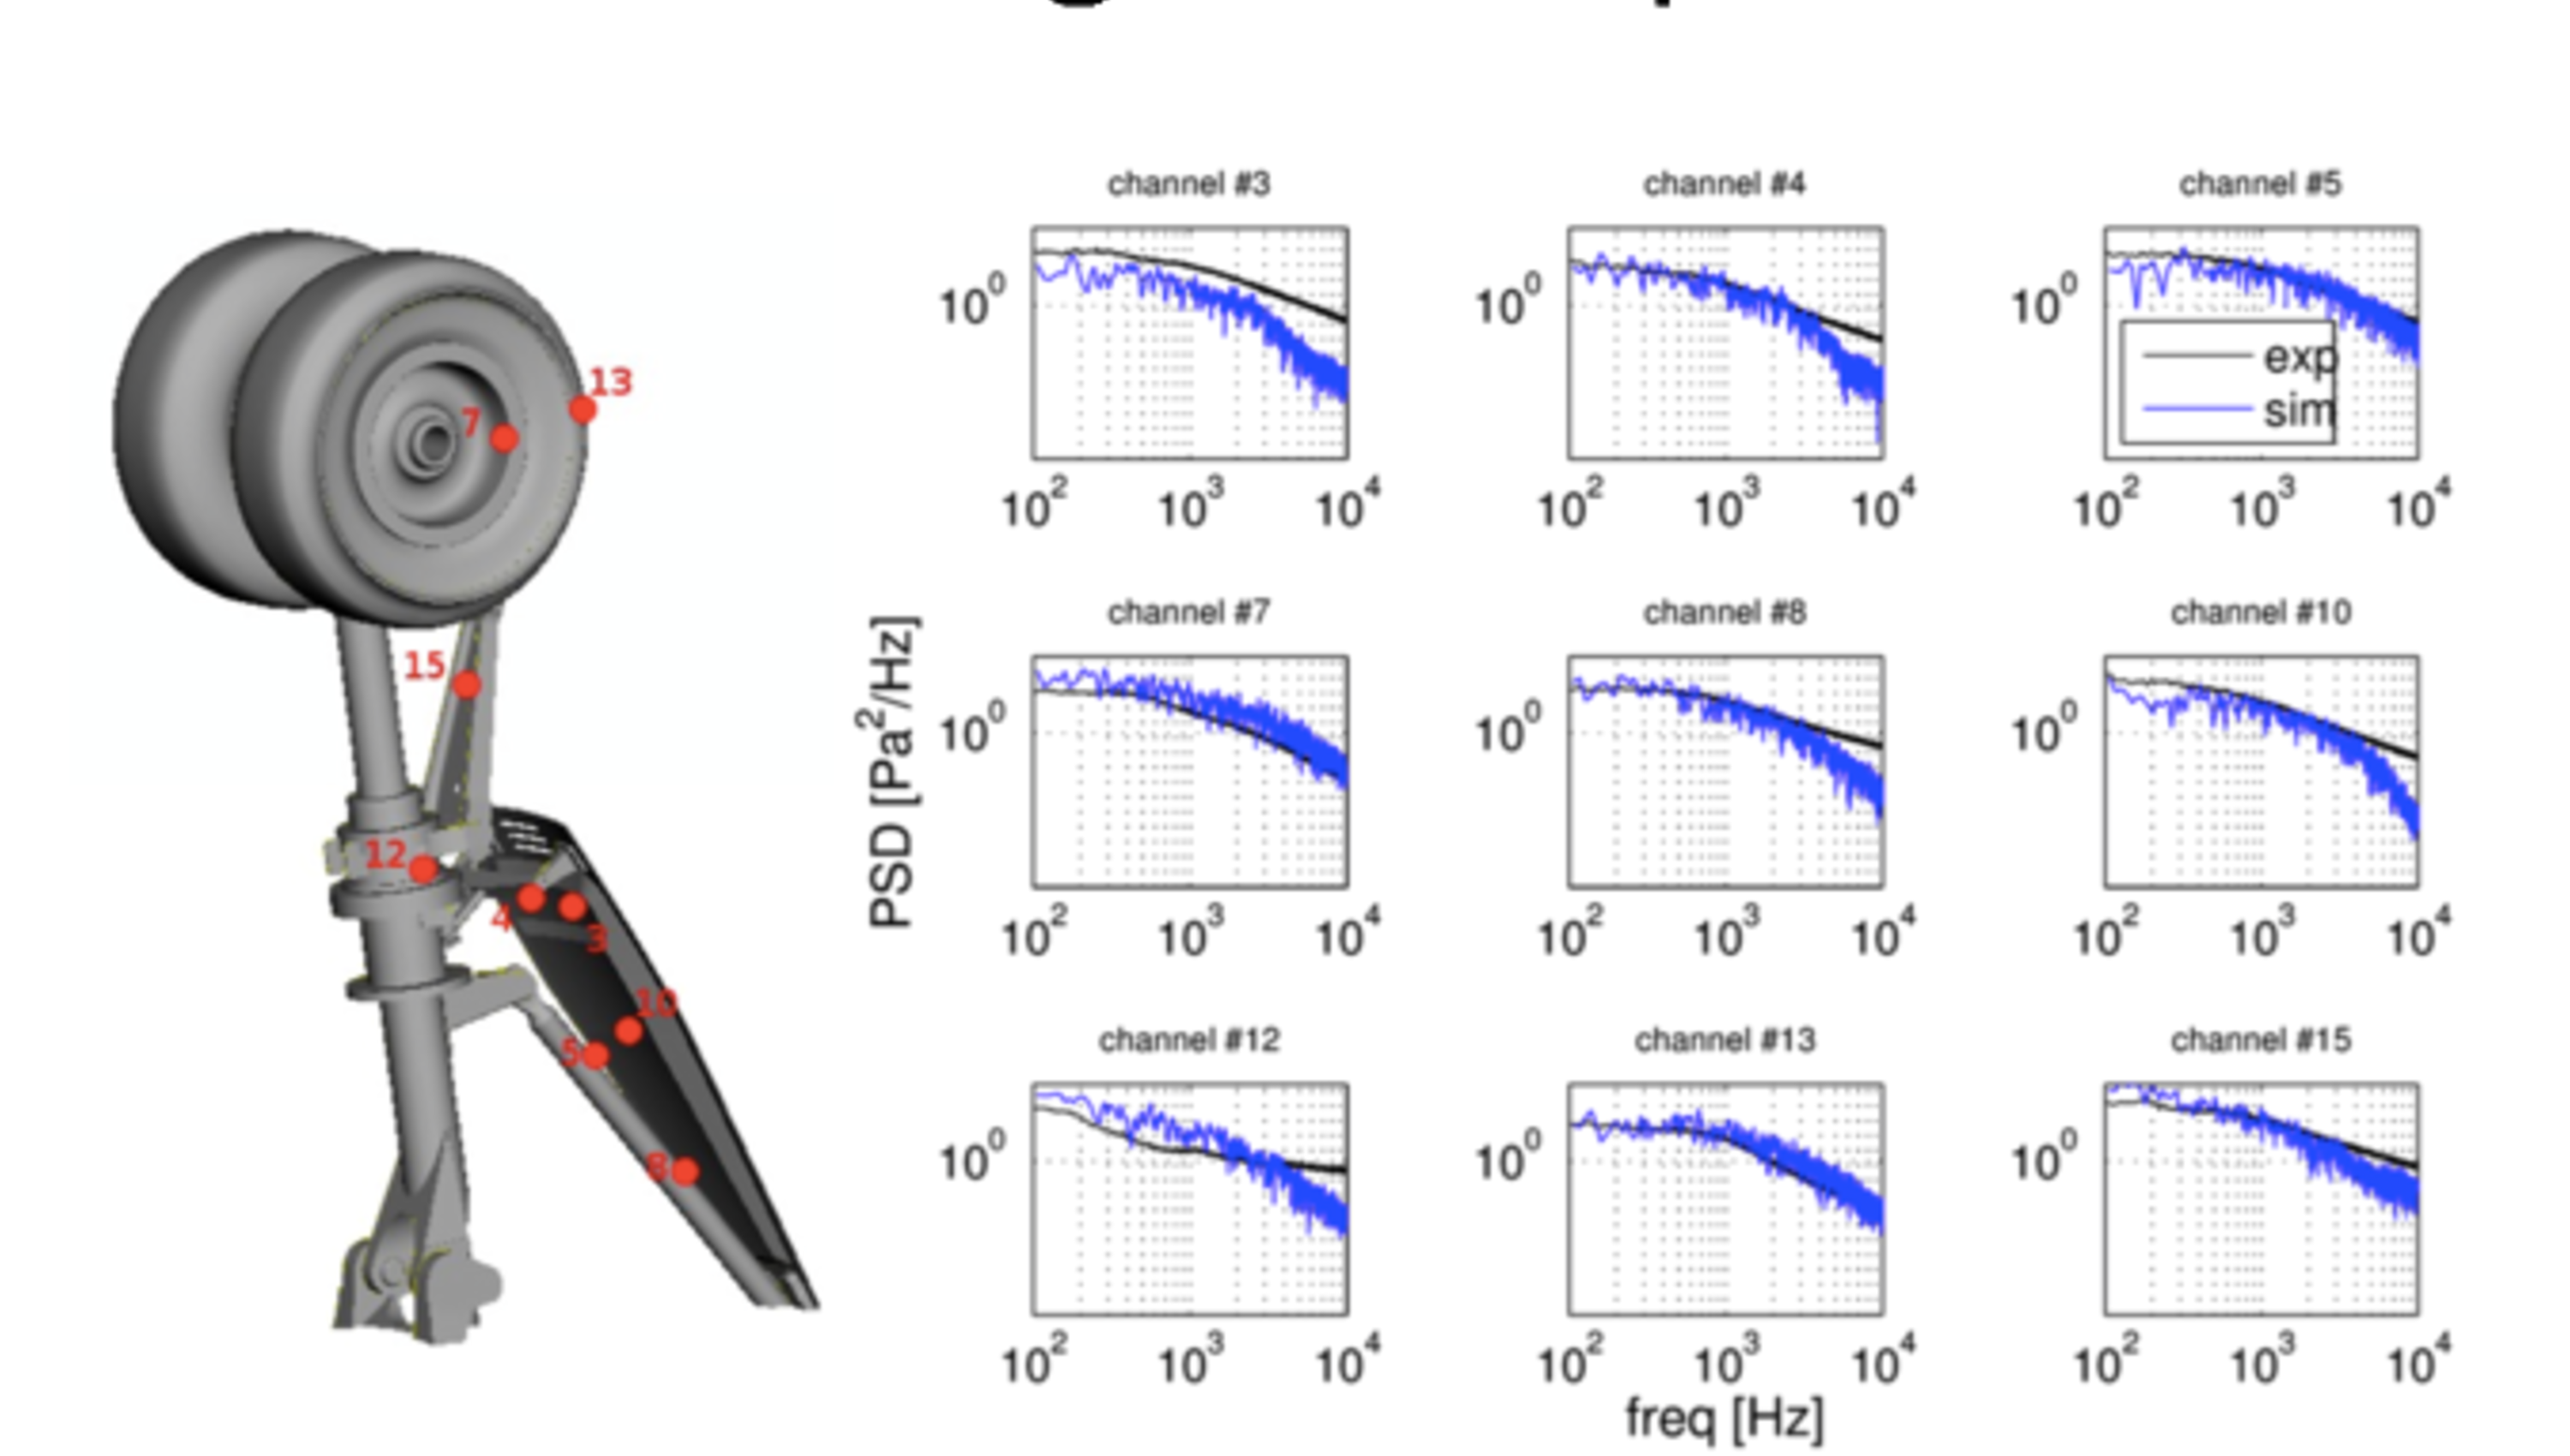
\includegraphics[width=10cm]{\figs/ctl/psd}
  \end{center}
  \caption{Sound pressure spectrum. Vilela De Abreu/N. Jansson/Hoffman, 18th AIAA Aeroacoustics Conference, 2012}
\end{figure}

Sampling pressure fluctuations at 44k hz: 1.4TB written for the sampling.

\end{frame}

%-----------------------------------------------------------------------------

\begin{frame}
  \frametitle{Example: Full Car Simulation}

\begin{figure}
  \begin{center}
    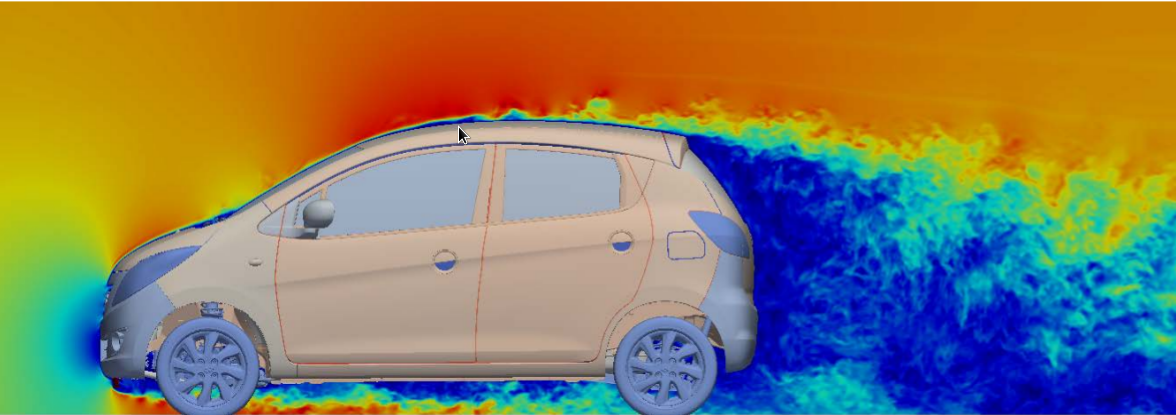
\includegraphics[width=10cm]{\figs/rikencar}
  \end{center}
  \caption{
    Full Car Simulation on the K-computer. Image from RIKEN AICS Website.
  }
\label{fig:manyone}
\end{figure}

\begin{itemize}
\item Building Cube Method (BCM) with immersed boundary
\item 32M cubes, and each cube $32^3$ cells
\item Surface resolution < 1 mm
\item Rotating wheels
\item $~50$TB per file uncompressed, $\approx1$TB per file compressed
\end{itemize}
\end{frame}

%-----------------------------------------------------------------------------

\begin{frame}
  \frametitle{MPI-IO}

\begin{itemize}
\item Part of the official MPI standard which covers parallel I/O.
\item Natural interface for expressing parallelism with collective I/O routines.
\item Opaque handling as the rest of MPI: simple and flexible.
\item Implementation details are hidden: lower-level can be optimized without modification of the solver code.
\end{itemize}

\end{frame}

\begin{frame}[fragile]

\frametitle{Example of simple code}
{\small
\begin{lstlisting}[style=c]
char mytext[BUF_LENGTH];
int rank,numtasks;
MPI_File fp;
MPI_Status status;
MPI_Offset offset;
// Initialize MPI
MPI_Init(&argc,&argv);
MPI_Comm_rank(MPI_COMM_WORLD,&rank);
MPI_Comm_size(MPI_COMM_WORLD,&numtasks);
sprintf(mytext,"Rank: %3d Hello World!\n",rank);
offset=rank*strlen(mytext);
// Open file and write text
MPI_File_open(MPI_COMM_WORLD,FILENAME,
              MPI_MODE_CREATE|MPI_MODE_WRONLY,
              MPI_INFO_NULL,&fp);
MPI_File_write_at(fp,offset,&mytext,strlen(mytext),
                  MPI_CHAR,&status);
MPI_File_close(&fp);
// Finalize MPI
MPI_Finalize();
\end{lstlisting}
}
\end{frame}

\begin{frame}[fragile]
\frametitle{MPI File Handle}

Before writing a MPI File handle needs to be created:
\begin{lstlisting}[style=c]
MPI_Comm    comm;
MPI_Info    info;
MPI_File    file;
MPI_File_open(comm, (char *) file, flag, info,
              &file);
\end{lstlisting}
with:
\begin{itemize}
\item \texttt{comm}: communicator for processes involved in the I/O
\item \texttt{info}: info object use to query information on the I/O
\item \texttt{flag}: mask to define the operation mode
\item \texttt{file}: file handle, note the address is passed for allocation
\end{itemize}

After I/O is done, the file handle can be closed:
\begin{lstlisting}[style=c]
MPI_File_close(&h.file);
\end{lstlisting}

\end{frame}

\begin{frame}[fragile]
\frametitle{MPI File Modes}

MPI-IO modes are a superset of POSIX modes:
{\small
\begin{lstlisting}[style=c]
/* MPIIO modes: POSIX */
MPI_MODE_RDONLY,           /*   0 ADIO_RDONLY */
MPI_MODE_RDWR,             /*   1 ADIO_RDWR  */
MPI_MODE_WRONLY,           /*   2 ADIO_WRONLY  */
MPI_MODE_CREATE,           /*   4 ADIO_CREATE */
MPI_MODE_EXCL,             /*   8 ADIO_EXCL */
/* MPIIO modes: MPI */
MPI_MODE_DELETE_ON_CLOSE,  /*  16 ADIO_DELETE_ON_CLOSE */
MPI_MODE_UNIQUE_OPEN,      /*  32 ADIO_UNIQUE_OPEN */
MPI_MODE_APPEND,           /*  64 ADIO_APPEND */
MPI_MODE_SEQUENTIAL,       /* 128 ADIO_SEQUENTIAL */
\end{lstlisting}
}
\end{frame}

\begin{frame}[fragile]
\frametitle{MPI File Modes}

MPI-IO modes are a superset of POSIX modes:
{\small
\begin{lstlisting}[style=c]
/* MPIIO modes: POSIX */
MPI_MODE_RDONLY,           /*   0 ADIO_RDONLY */
MPI_MODE_RDWR,             /*   1 ADIO_RDWR  */
MPI_MODE_WRONLY,           /*   2 ADIO_WRONLY  */
MPI_MODE_CREATE,           /*   4 ADIO_CREATE */
MPI_MODE_EXCL,             /*   8 ADIO_EXCL */
/* MPIIO modes: MPI */
MPI_MODE_DELETE_ON_CLOSE,  /*  16 ADIO_DELETE_ON_CLOSE */
MPI_MODE_UNIQUE_OPEN,      /*  32 ADIO_UNIQUE_OPEN */
MPI_MODE_APPEND,           /*  64 ADIO_APPEND */
MPI_MODE_SEQUENTIAL,       /* 128 ADIO_SEQUENTIAL */
\end{lstlisting}
}
\end{frame}

\begin{frame}[fragile]
\frametitle{MPI File Modes}

POSIX-like modes have same semantics:\\[2ex]
\begin{center}
\begin{tabular}{ll}
\hline
\texttt{MPI\_MODE\_RDONLY} & Read-only\\
\texttt{MPI\_MODE\_RDWR}   & Read/Write\\
\texttt{MPI\_MODE\_WRONLY} & Write only\\
\texttt{MPI\_MODE\_CREATE} & Create if file exists\\
\texttt{MPI\_MODE\_EXCL}   & Error if file exists\\
\hline
\end{tabular}
\end{center}

MPI-IO modes:\\[2ex]
\begin{tabular}{ll}
\hline
\texttt{MPI\_MODE\_DELETE\_ON\_CLOSE} & Delete file on close\\
\texttt{MPI\_MODE\_UNIQUE\_OPEN}      & Only by MPI process (not even outside)\\
\texttt{MPI\_MODE\_APPEND}            & Append to existing file\\
\texttt{MPI\_MODE\_SEQUENTIAL}        & Sequential mode for backup devices\\
\hline
\end{tabular}

\end{frame}

\begin{frame}[fragile]
\frametitle{MPI File Write}

A simple write operation using the file handle could be to write a chunk of vector of global size $N$ distributed uniformly on all the processes:
{\small
\begin{lstlisting}[style=c]
MPI_Offset mysize = N/size;
MPI_File_seek (fh , rank* mysize * sizeof ( double ),
MPI_SEEK_SET );
MPI_File_write (fh , vec , mysize , MPI_DOUBLE ,
MPI_STATUS_IGNORE );
\end{lstlisting}

\medskip
Note the seek call to position the file pointer to the right offset.

\medskip
The equivalent collective operation:
\begin{lstlisting}[style=c]
MPI_File_write_all (fh , vec , mysize , MPI_DOUBLE ,
                    MPI_STATUS_IGNORE );
\end{lstlisting}
}
\end{frame}

\begin{frame}[fragile]
\frametitle{MPI File Write}

To save MPI call to seek, the offset can be managed externally:
\begin{lstlisting}[style=c]
MPI_Offset mysize = N/size;
MPI_Offset offset = rank * mysize * sizeof(double);
MPI_File_write_at_all(fh, offset, vec , mysize ,
                   MPI_DOUBLE , MPI_STATUS_IGNORE );
\end{lstlisting}
Note that the offset is in bytes.

\medskip
Remember that each process usually owns a range of entities (that needs to be written) but also ghosted entities that are copies of entities owned by other processes (that should not be written).

\end{frame}

\begin{frame}[fragile]
\frametitle{Example of code in DOLFIN-HPC}

We are going through classes implemented for DOLFIN-HPC:
\begin{itemize}
\item Binary file write with MPI-IO
\item ASCII XML file write with MPI-IO
\end{itemize}

\medskip
It is a good practice to design an interface for your software package so that parallel I/O is handled transparently.

\end{frame}

\begin{frame}[fragile]
\frametitle{Writing a vector with MPI-IO}
First step is to extract information about the range of owned data:
{\small
\begin{lstlisting}[style=c]
GenericVector x;
uint size = x.local_size();
real *values = new real[size];
uint offset[2] = { 0, 0 };
offset[0] = x.offset();
offset[1] = size;
x.get(values);
\end{lstlisting}
}

The library specifies a format for reading/writing to specify for instance the number of processes:
{\small
\begin{lstlisting}[style=c]
BinaryFileHeader hdr;
uint pe_rank = MPI::rank();
hdr.magic = BINARY_MAGIC;
hdr.pe_size = MPI::size();
hdr.type = BINARY_VECTOR_DATA;
\end{lstlisting}
}

\end{frame}

\begin{frame}[fragile]
\frametitle{Writing a vector with MPI-IO}

Writing a file header containing metadata:
{\scriptsize
\begin{lstlisting}[style=c]
MPI_File fh;
MPI_Offset byte_offset;
MPI_File_open(dolfin::MPI::DOLFIN_COMM, (char *) filename.c_str(),
              MPI_MODE_WRONLY | MPI_MODE_CREATE, MPI_INFO_NULL, &fh);
MPI_File_write_all(fh, &hdr, sizeof(BinaryFileHeader),
                   MPI_BYTE, MPI_STATUS_IGNORE);
byte_offset = sizeof(BinaryFileHeader);
\end{lstlisting}
}

Writing range of each process:
{\scriptsize
\begin{lstlisting}[style=c]
MPI_File_write_at_all(fh, byte_offset + pe_rank * 2 * sizeof(uint),
                      &offset[0], 2, MPI_UNSIGNED, MPI_STATUS_IGNORE);
byte_offset += hdr.pe_size * 2 * sizeof(uint);
\end{lstlisting}
}

Writing contiguous array:
{\scriptsize
\begin{lstlisting}[style=c]
MPI_File_write_at_all(fh, byte_offset + offset[0] * sizeof(real), values,
                      offset[1], MPI_DOUBLE, MPI_STATUS_IGNORE);
MPI_File_close(&fh);

delete[] values;
\end{lstlisting}
}

\end{frame}

\begin{frame}[fragile]
\frametitle{Using MPI Data Types}

In the lecture notes several examples are given using MPI derived data types, and is useful for example when writing strided data, with a given data packing.

\medskip
In practice, using MPI derived data types is a good way to write error prone code in an elegant way and will simplify the structure of the implementation.


\end{frame}

\end{document}

